\chapter{مقدمه}

\section{تعمیر و نگهداری}

در دنیای نوین امروز، وابستگی به فناوری و صنایع مختلف برای ارائه خدمات و تولید محصولات مورد نیاز بشدت افزایش یافته‌است. در نتیجه این افزایش، تعداد کارخانه‌ها و تجهیزات برای رفع این نیازها نیز افزایش یافته‌است. همه تجهیزات و وسایل پس از استفاده زیاد دچار نقص و فراوانی می‌شوند. خرابی تجهیزات در کارخانه‌ها و حطوط تولید پدیده‌ای نامطلوب است. خرابی تجهیزات باعث ایست خط تولید و وارد کردن ضرر مالی به صاحبان کارخانه‌ها خواهد شد. به‌همین دلیل، تعمیر و نگهداری تجهیزات اهمیت بالایی دارد. 

سیاست‌های انجام تعمیرات و نگهداری به سه دسته اصلی تقسیم می‌شوند؛ که در \cref{MS} آورده شده‌است:

\begin{figure}[!h]
\centering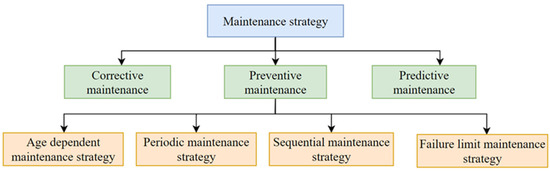
\includegraphics[scale=1]{maintenance_strategy.png}
\caption{سیاست‌های انجام تعمیرات و نگهداری\cite{zhao2022review}}\label{MS}
\end{figure}

این سیاست‌ها عبارتند از:
\begin{itemize}
\item نگهداری اصلاحی\LTRfootnote{Corrective Maintenance}: این نوع نگهداری با اتفاق افتادن خرابی رخ می‌دهد و تنها در صورت خرابی قطعه تعمیر انجام می‌شود. همانطور که مشخص است در این حالت روند کارکرد عادی متوقف می‌شود: به‌علاوه، در این حالت تعمیر می‌تواند با تاخیر انجام شود زیرا ممکن است در لحظه قطعات مورد نیاز برای تعمیر موجود نباشد. از این سیاست بیشتر به‌عنوان مکملی برای سیاست‌های بعدی استفاده می‌شود\cite{zhao2022review}.

\item نگهداری پیش‌گیرانه\LTRfootnote{Preventive Maintenance}: در این حالت، نگهداری و تعمیر بر اساس رابطه بین نرخ خرابی، توزیع زمان خرابی و سایر آستانه‌هایی که از تعداد زیادی از آمارهای خرابی بدست می‌آید زمان‌بندی می‌شود. در واقع در این نوع نگهداری هدف کاهش احتمال خرابی قطعات است. این نوع نگهداری با توجه به نوع اطلاعات به سیاست‌های وابسته عمر،\LTRfootnote{Age Dependent Strategies} سیاست‌های دوره‌ای\LTRfootnote{Periodic Strategies}، سیاست‌های ترتیبی\LTRfootnote{Sequential Strategies} و سیاست‌های محدودکننده خرابی\LTRfootnote{Failure Limited Strategies} تقسیم می‌شوند\cite{zhao2022review}.

\item نگهداری پیش‌بینانه\LTRfootnote{Predictive Maintenance}: این نوع نگهداری بر روند کاهش کارایی قطعات با استفاده از وضعیت آنها نظارت کرده، وضعیت آنها را در آینده پیش‌بینی می‌کند و مداوم برنامه تعمیر و نگهداری را بروزرسانی می‌کند، تا اینکه شرایط توقف بروزرسانی برآورده شود. با توجه به این ویژگی، این سیاست فقط برای تجهیزاتی که وضعیت آنها قابل نظارت است می‌تواند استفاده شود\cite{zhao2022review}.
\end{itemize} 

\section{تعریف مسئله}

\section{مطالب پایان‌نامه را چطور بنویسم؟}
\subsection{نوشتن فصل‌ها}
همان‌طور که در بخش 
\ref{sec2}
گفته شد، برای جلوگیری از شلوغی و سردرگمی کاربر در هنگام حروف‌چینی، قسمت‌های مختلف پایان‌نامه از جمله فصل‌ها، در فایل‌های جداگانه‌ای قرار داده شده‌اند. 
بنابراین، اگر می‌خواهید مثلاً مطالب فصل ۱ را تایپ کنید، باید فایل‌های 
\verb;AUTthesis.tex;
و
\verb;chapter1;
را باز کنید و محتویات داخل فایل 
\verb;chapter1;
را پاک کرده و مطالب خود را تایپ کنید. توجه کنید که همان‌طور که قبلاً هم گفته شد، تنها فایل قابل اجرا، فایل 
\verb;AUTthesis.tex;
است. لذا برای دیدن حاصل (خروجی) فایل خود، باید فایل  
\verb;chapter1;
را 
\verb;Save;
کرده و سپس فایل 
\verb;AUTthesis.tex;
را اجرا کنید. یک نکته بدیهی که در اینجا وجود دارد، این است که لازم نیست که فصل‌های پایان‌نامه را به ترتیب تایپ کنید. می‌توانید ابتدا مطالب فصل ۳ را تایپ کنید و سپس مطالب فصل ۱ را تایپ کنید.

نکته بسیار مهمی که در اینجا باید گفته شود این است که سیستم
\lr{\TeX},
محتویات یک فایل تِک را به ترتیب پردازش می‌کند. به عنوان مثال، اگه فایلی، دارای ۴ خط دستور باشد، ابتدا خط ۱، بعد خط ۲، بعد خط ۳ و در آخر، خط ۴ پردازش می‌شود. بنابراین، اگر مثلاً مشغول تایپ مطالب فصل ۳ هستید، بهتر است
که دو دستور
\verb~\chapter{مقدمه}

\section{تعمیر و نگهداری}

در دنیای نوین امروز، وابستگی به فناوری و صنایع مختلف برای ارائه خدمات و تولید محصولات مورد نیاز بشدت افزایش یافته‌است. در نتیجه این افزایش، تعداد کارخانه‌ها و تجهیزات برای رفع این نیازها نیز افزایش یافته‌است. همه تجهیزات و وسایل پس از استفاده زیاد دچار نقص و فراوانی می‌شوند. خرابی تجهیزات در کارخانه‌ها و حطوط تولید پدیده‌ای نامطلوب است. خرابی تجهیزات باعث ایست خط تولید و وارد کردن ضرر مالی به صاحبان کارخانه‌ها خواهد شد. به‌همین دلیل، تعمیر و نگهداری تجهیزات اهمیت بالایی دارد. 

سیاست‌های انجام تعمیرات و نگهداری به سه دسته اصلی تقسیم می‌شوند؛ که در \cref{MS} \cite{zhao2022review} آورده شده‌است:

\begin{figure}[!h]
\centering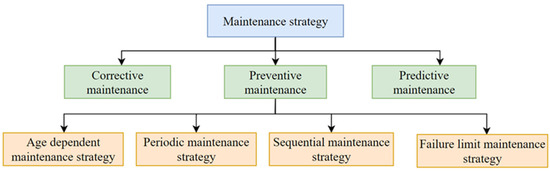
\includegraphics[scale=1]{maintenance_strategy.png}
\caption{سیاست‌های انجام تعمیرات و نگهداری}\label{MS}
\end{figure}

این سیاست‌ها عبارتند از:
\begin{itemize}
\item نگهداری اصلاحی\LTRfootnote{Corrective Maintenance}: این نوع نگهداری با اتفاق افتادن خرابی رخ می‌دهد و تنها در صورت خرابی قطعه تعمیر انجام می‌شود. همانطور که مشخص است در این حالت روند کارکرد عادی متوقف می‌شود: به‌علاوه، در این حالت تعمیر می‌تواند با تاخیر انجام شود زیرا ممکن است در لحظه قطعات مورد نیاز برای تعمیر موجود نباشد. از این سیاست بیشتر به‌عنوان مکملی برای سیاست‌های بعدی استفاده می‌شود\cite{zhao2022review}.

\item نگهداری پیش‌گیرانه\LTRfootnote{Preventive Maintenance}: در این حالت، نگهداری و تعمیر بر اساس رابطه بین نرخ خرابی، توزیع زمان خرابی و سایر آستانه‌هایی که از تعداد زیادی از آمارهای خرابی بدست می‌آید زمان‌بندی می‌شود. در واقع در این نوع نگهداری هدف کاهش احتمال خرابی قطعات است. این نوع نگهداری با توجه به نوع اطلاعات به سیاست‌های وابسته عمر،\LTRfootnote{Age Dependent Strategies} سیاست‌های دوره‌ای\LTRfootnote{Periodic Strategies}، سیاست‌های ترتیبی\LTRfootnote{Sequential Strategies} و سیاست‌های محدودکننده خرابی\LTRfootnote{Failure Limited Strategies} تقسیم می‌شوند\cite{zhao2022review}.

\item نگهداری پیش‌بینانه\LTRfootnote{Predictive Maintenance}: این نوع نگهداری بر روند کاهش کارایی قطعات با استفاده از وضعیت آنها نظارت کرده، وضعیت آنها را در آینده پیش‌بینی می‌کند و مداوم برنامه تعمیر و نگهداری را بروزرسانی می‌کند، تا اینکه شرایط توقف بروزرسانی برآورده شود. با توجه به این ویژگی، این سیاست فقط برای تجهیزاتی که وضعیت آنها قابل نظارت است می‌تواند استفاده شود\cite{zhao2022review}.
\end{itemize} 

\section{راهکار پیشنهادی}

با توجه به اهمیت نگهداری و نقش نگهداری اصولی در کاهش هزینه، در این پروژه به ایجاد چارچوبی مناسب برای ارائه راهکاری بر مبنای سیاست نگهداری پیش‌بینانه می‌پردازیم. یکی از نیازهای این سیاست حجم زیادی از داده جمع‌آوری شده از وضعیت تجهیزات برای پیش‌بینی دقیق است. در این پروژه در بستر اینترنت اشیاء\LTRfootnote{Internet of Things} داده‌های لرزش با استفاده از سنسور \lr{MEMS}\LTRfootnote{Micro Electric Mechanical Sensor} جمع‌آوری شده و در زمان‌های مشخص با استفاده از پروتکل زیگبی\LTRfootnote{Zigbee Protocol} برای دروازه\LTRfootnote{Gateway} فرستاده می‌شود. پس از جمع‌آوری حجم مشخصی از داده‌هااطلاعات برای پردازش بیشتر به سرور فرستاده می‌شوند. در انتها نیز اطلاعات پردازش‌شده و تخمین عمر مفید باقیمانده\LTRfootnote{Remaining Useful Lifetime(RUL)} در یک صفحه وب نمایش داده می‌شود.

\section{کارهای مشابه}
در \cite{tinga2010application} مدلی برای خرابی قطعات مبتنی بر میزان استفاده از تجهیزات و بار داخلی آنها ارائه شده‌است اما مدل ارائه‌شده محدود به یک مدل تجهیزات است و برای استفاده در سایر مدل‌ها نظارت مجدد لازم است. در \cite{wu2007neural} رویکردی مبتنی بر شبکه عصبی جهت پیش‌بینی عمر مفید باقیمانده تجهیزات چرخشی ارائه شده‌است اما تنها مختص به این دسته از تجهیزات است. در \cite{kaiser2009predictive} رویکردی مبتنی بر شبکه عصبی جهت پیش‌بینی زمان نگهداری و تعمیرات تجهیزات بر اساس مدل خرابی و کارایی آنها ارائه می‌شود اما در یک محیط شبیه‌سازی‌شده و کنترل‌شده آزمایش شده‌است و در هنگام استفاده در محیط واقعی غیرعملی است.

بطور کلی در پژوهش‌های یادشده رویکرد‌های ارائه‌شده مختص نوع خاصی از تجهیزات است و در یک مجیط آزمایشگاهی و کنترل‌شده ارزیابی شده‌اند. در حالیکه در این پروژه با استفاده از داده‌های جمع‌آوری‌شده از قطعات مختلف سعی کرده‌ایم رویکردی کلی و مناسب محیط واقعی و صنعتی ارائه دهیم.
~
و
\verb~\chapter{طریقه‌ی مرجع نویسی و واژه‌نامه‌}
\section{طریقه‌ی مرجع نویسی}
برای نوشتن مراجع پایان نامه، برای راحتی کار به صورت زیر عمل می‌کنیم:
\subsection{بارگیری مراجع}
در ابتدا مراجع را باید از سایت‌های معتبر بارگیری کنیم، مثلا برای ارجاع دادن به مقاله‌ی
\lr{A classification of some Finsler connections and their applications}
ابتدا به سایت
\href{scholar.google.com}{گوگل اسکولار} 
رفته و این مقاله را جستجو می‌کنیم. پس از پیدا کردن این مقاله، مانند شکل زیر، در زیر نام و چکیده‌ی مقاله، $5$ گزینه وجود دارد که عبارتند از:\\

\begin{enumerate}
\item \lr{ Cited by}

\item \lr{ Related articles}

\item \lr{ All 6 versions}

\item \lr{ Cite}

\item \lr{ Save}
\end{enumerate}
\begin{figure}[!h]
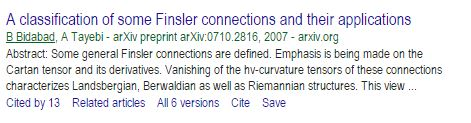
\includegraphics[height=3cm]{bidabad}
\caption{نمونه یک مقاله در گوگل اسکولار}
\end{figure}
در اینجا ما به گزینه‌ی چهارم یعنی
\lr{ Cite}
احتیاج داریم. بر روی آن کلیک کرده و پنجره‌ای مانند
\cref{fig.2}
باز می‌شود که دارای $4$ گزینه‌ی زیر است:
\begin{enumerate}
\item \lr{BibTeX}

\item \lr{EndNote}

\item \lr{RefMan}

\item \lr{RefWorks}
\end{enumerate}
\begin{figure}
\centering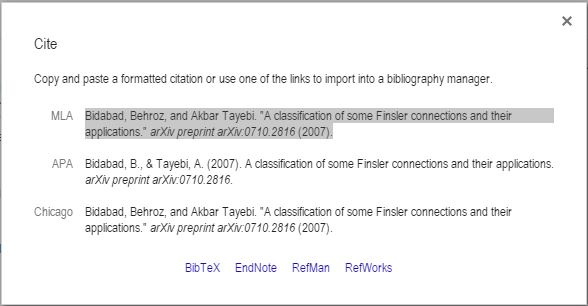
\includegraphics[scale=.6]{bibref}
\caption{پنجره‌ی باز شده در گوگل اسکولار}\label{fig.2}
\end{figure}
روی گزینه‌ی اول، یعنی
\verb;BibTeX;
کلیک کرده و همه‌ی نوشته‌های پنجره‌ی باز شده را مانند زیر، کپی کرده و در فایل
\verb;references.bib;
موجود در فایل
\verb;AUTthesis;
پیست می‌کنیم. سپس کلیدهای
\verb;Ctrl+s;
را می‌زنیم تا فایل ذخیره شود.\\
\begin{latin}
	\normalsize
\begin{verbatim}
@ article{bidabad2007classification,
title={A classification of some Finsler connections and their applications},
author={Bidabad, Behroz and Tayebi, Akbar},
journal={arXiv preprint arXiv:0710.2816},
year={2007}
}
\end{verbatim}
\end{latin}
\subsection{روش ارجاع در متن}
برای ارجاع دادن به مقاله‌ی بالا، باید در جایی که می‌خواهید ارجاع دهید، دستور زیر را تایپ کنید:
\begin{latin}
\lr{$\backslash$cite\{bidabad2007classification\}}
\end{latin}
همانطور که مشاهده می‌کنید از کلمه‌ای که در سطر اول ادرس مقاله آمده (یعنی کلمه‌ی پس از
\lr{@article$\lbrace$})
استفاده کرده‌ایم. پس از دستور فوق، به صورت \cite{bidabad2007classification} و \cite{aa} مرجع خواهد خورد. توجه شود که در صورتی مراجع چاپ خواهند شد که در متن به انها ارجاع داده شده باشد. همچنین برای ارجاع چندتایی از دستور 
\lr{$\backslash$cite\{name1, name2,...\}}
استفاده کنید که به‌صورت \cite{najafi2008finsler, zakeri, najafi} ارجاع خواهند خورد.
\subsection{روش اجرای برنامه}
ابتدا فایل
\verb;AUT_thesis.tex;
را باز کرده و آن را دو بار اجرا کنید. سپس حالت اجرا را از 
\verb;Build Quick;
به حالت
\verb;Bibtex;
تغییر داده و دوباره برنامه را اجرا کنید. دو بار دیگر برنامه را در حالت 
\verb;Build Quick;
اجرا کرده و نتیجه را مشاهده کنید. در این روش تمامی مراجع بر اساس اینکه کدام یک در متن زودتر به آن ارجع داده شده لیست خواهند شد.
\subsection{مراجع فارسی}
برای نوشتن مراجع فارسی باید به صورت دستی، در همان فایل قبلی به صورت زیر عمل می‌کنیم:
\begin{LTR}
\noindent\verb;@article{manifold,;\\
\verb;title={;منیفلد هندسه\verb;},;\\
\verb;author={;بیدآباد دکتربهروز \verb;},;\\
\verb;journal{; امیرکبیر صنعتی دانشگاه\verb;},;\\
\verb;year={1389},;\\
\verb;LANGUAGE={Persian};\\
\verb;};
\end{LTR}
همانطور که مشاهده می‌کنید تنها تفاوت آن با حالت مراجع انگلیسی، سطر آخر آن می‌باشد که زبان را مشخص می‌کند که حتماً باید نوشته شود.
\section{راهنمای واژه‌نامه}

به دلیل پیچیدگی واژه‌نامه‌های موجود در سایت پارسی لاتک، از روش زیر برای نوشتن واژه‌نامه استفاده کنید:

ابتدا با استفاده از اکسل، واژه های خود را یک‌بار براساس حروف الفبای فرسی و بار دیگر انگلیسی مرتب کنید. سپس واژه ها را در فایل \lr{dicen2fa} و \lr{dicfa2en} قرار دهید.

\section{ساخت نمایه}\label{Namaye}
\subsection{ساخت نمایه}
 \begin{enumerate}

\item
کلمات مورد نظر خود مثلا \lr{word} با دستور \verb|\index{word}| ایندکس کنید.
\item
نحوه‌ی اجرای \lr{Make Index}   در ویرایشگرهای \lr{TeX Maker} و \lr{TeX Works}:
\begin{itemize}
\item  تک‌میکر: از منوی \lr{Tools} گزینه‌ی \lr{Xindy Make Index} را کلیک کنید یا از دکمه‌‌های میانبر \lr{Ctrl+Alt+I} استفاده کنید.

\item  تک‌ورکز: ابتدا باید مثل عکس زیر تنظیم  و سپس گزینه‌ی \lr{Xindy Make Index}  انتخاب و روی دکمه‌ی سبز رنگ کلیک کنید یا از دکمه‌های  \lr{Ctrl+T} استفاده کنید.

\begin{figure}[!h]
\centerline{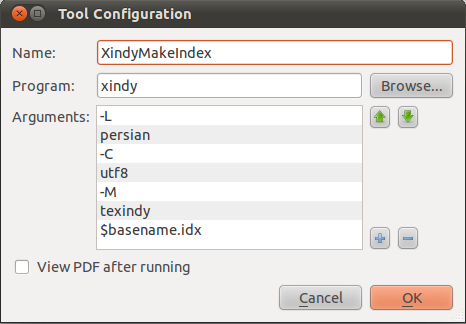
\includegraphics[width=.5\textwidth]{Xindy_Make_Index.png}}
\caption{تنظیمات مربوط به تک‌ورکز}
\end{figure}

\end{itemize}
 \end{enumerate}
 
 \index{کتاب}
\index{پارسی‌لاتک}
\index{بی‌دی}
\index{سوال}
\index{عنصر}
\index{گزینه}
\index{ژاکت}
\index{مرکز دانلود}
\index{اجرا}
\index{تک‌لایو}
\index{ثالث}
\index{جهان}
\index{چهار}
\index{حمایت}
\index{خواهش}
\index{دنیا}
\index{زی‌پرشین}
\index{ریحان}
\index{شیرین}
\index{صمیمی}
\index{ضمیر}
\index{طبیب}~
را در فایل 
\verb~AUTthesis.tex~،
غیرفعال%
\RTLfootnote{
برای غیرفعال کردن یک دستور، کافی است پشت آن، یک علامت
\%
 بگذارید.
}
 کنید. زیرا در غیر این صورت، ابتدا مطالب فصل ۱ و ۲ پردازش شده (که به درد ما نمی‌خورد؛ چون ما می‌خواهیم خروجی فصل ۳ را ببینیم) و سپس مطالب فصل ۳ پردازش می‌شود و این کار باعث طولانی شدن زمان اجرا می‌شود. زیرا هر چقدر حجم فایل اجرا شده، بیشتر باشد، زمان بیشتری هم برای اجرای آن، صرف می‌شود.

\subsection{مراجع}
برای وارد کردن مراجع به فصل 2
مراجعه کنید.
\subsection{واژه‌نامه فارسی به انگلیسی و برعکس}
برای وارد کردن واژه‌نامه فارسی به انگلیسی و برعکس، بهتر است مانند روش بکار رفته در فایل‌های 
\verb;dicfa2en;
و
\verb;dicen2fa;
عمل کنید.

\section{اگر سوالی داشتم، از کی بپرسم؟}
برای پرسیدن سوال‌های خود در مورد حروف‌چینی با زی‌پرشین،  می‌توانید به
 \href{http://forum.parsilatex.com}{تالار گفتگوی پارسی‌لاتک}%
\LTRfootnote{\url{http://www.forum.parsilatex.com}}
مراجعه کنید. شما هم می‌توانید روزی به سوال‌های دیگران در این تالار، جواب بدهید.
